\documentclass[../main.tex]{subfiles}

\begin{document}

\subsection{Writing time VS offset}
\begin{figure}[h]
    \centering
    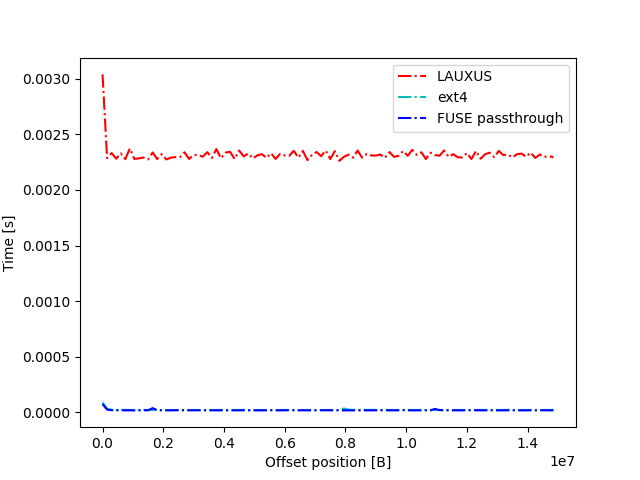
\includegraphics[width=\textwidth]{images/appendix/per_offset_write}
    
    \caption{Small offset edition into a 15MB file at different index}
    \label{appendix:figure:per_offset_write}
\end{figure}
\par From analysing the Section \ref{section:analysis:write_offset_overhead}, we want to be sure that our implementation is correct. In more details, we want to be sure that, for fixed file size, writing a few bytes takes the same amount of time no matter the offset. This expectation seems trivial by analysing our theoretical model but an incorrect implementation could end up giving different results. By analysing the Figure \ref{appendix:figure:per_offset_write}, we clearly see that our implementation is correct (for this functionality at least).

\end{document}